\subsection{Analys} \label{sec:analysis}

\subsubsection{Detektorns känslighet} \label{sec:sensitivity}

I figur~\ref{fig:sensitivityraw} visas uppmätta värden på detektorns
känslighet \parencite{instructions}. Mätningarna har utförts genom ett
kalibreringsprov vars aktivitet är känt. Figuren visar mätdatapunkter
och en anpassad kurva.

\begin{figure}[!ht]
    \centering
    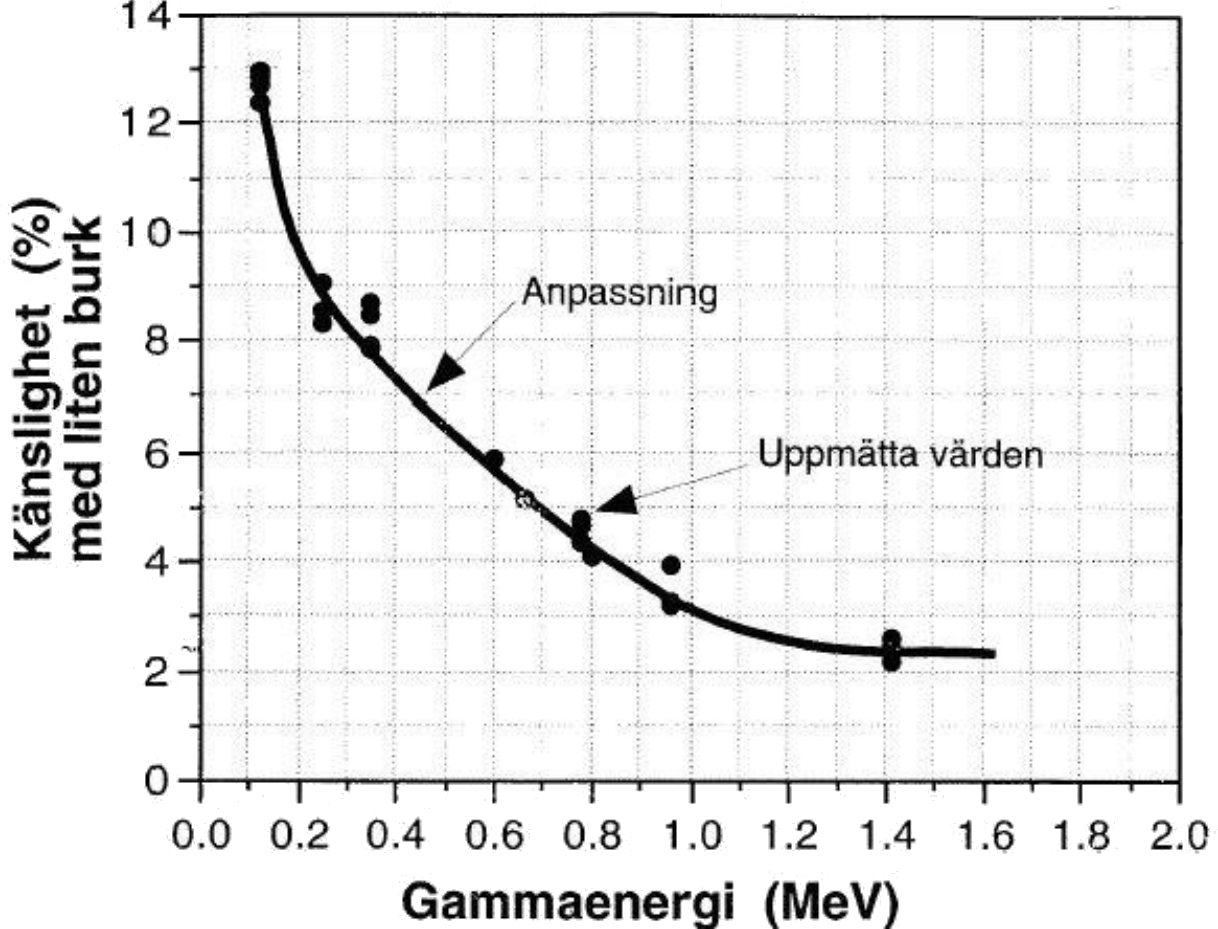
\includegraphics[width=\textwidth, keepaspectratio]{../images/sensitivity_raw.png}
    \caption{
        Detektorns känslighet vid olika energinivåer beräknad genom
        kalibreringsprov, men mätdatapunkter och anpassningskurva.
    }
    \label{fig:sensitivityraw}
\end{figure}

Då varken kurvans funktion eller mätvärdena är givna kan inga exakta värden
avläsas. Dock visas i avsnitt~\ref{sec:measurements} att topparna i de båda
gammaspektrumen har relativt låg fördelning. Av denna anledning har funktionen
approximerats linjärt i utvalda intervall. För svampprovet, vars topp ligger i
intervallet \qtyrange{0.58}{0.75}{\MeV}, har linjen passats till punkterna
\point{0.60}{5.6} och \point{0.70}{5.0}. För saltprovet, vars topp ligger i
intervallet \qtyrange{1.38}{1.54}{\MeV}, har den passats till \point{1.4}{2.4}
och \point{1.55}{2.4}. Två värdesiffror har valts då ingen högra precision kan
utläsas av enbart bilden. Notera att den vertikala axeln i
figur~\ref{fig:sensitivityraw} anges i \unit{\percent}. Linjerna $L_1$
respektive $L_2$ fås då av energin $E$ enligt:
%
\begin{align}
    L_1 &= \num{-0.06} E + \num{0.092} \label{eq:line1} \\
    L_2 &= \num{0.024}                 \label{eq:line2}
\end{align}
%
Dessa punkter, och linjerna de ger upphov till, visas tillsammans med
anpassningen i figur~\ref{fig:sensitivity}.

\begin{figure}[!ht]
    \centering
    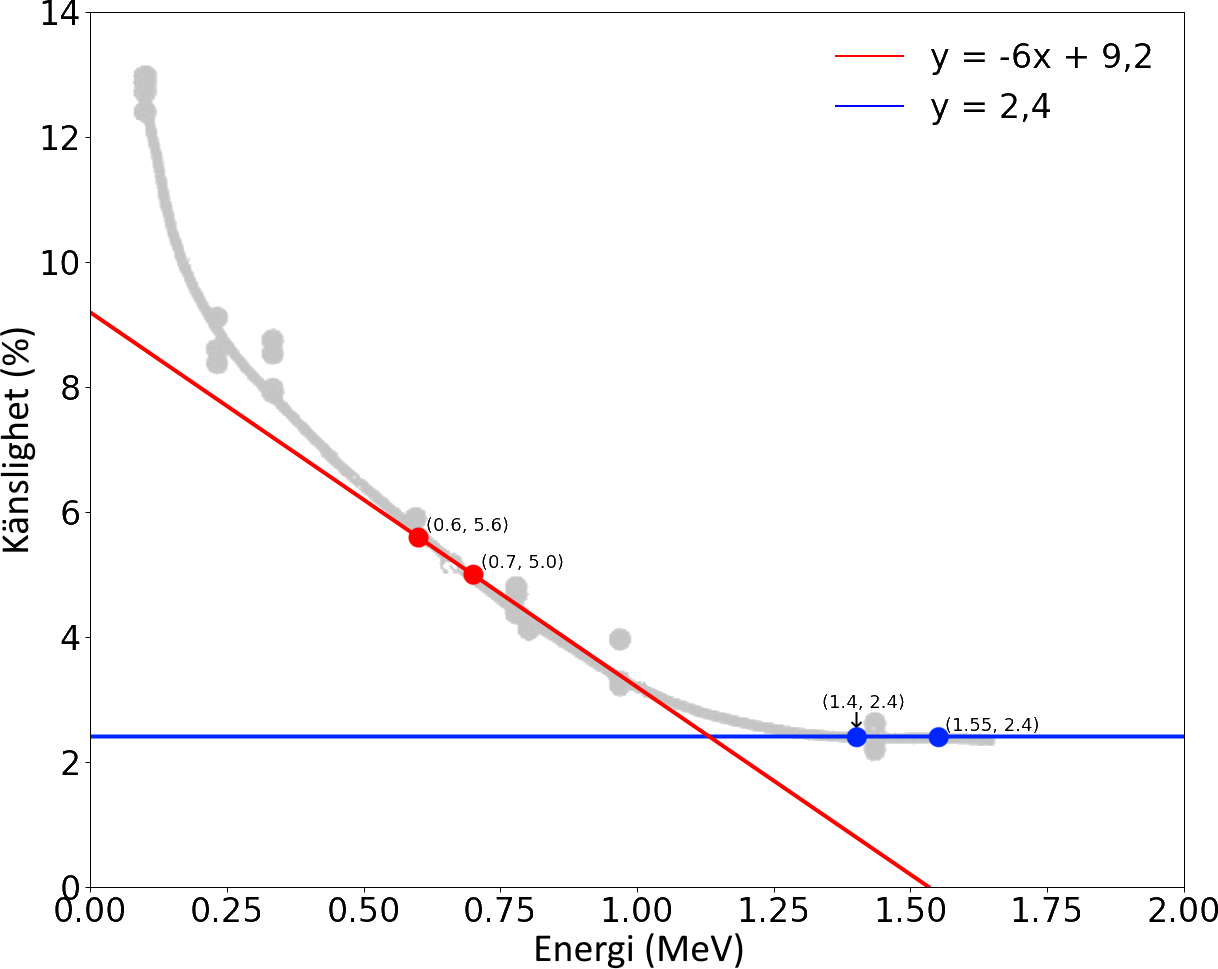
\includegraphics[width=\textwidth, keepaspectratio]{../images/sensitivity.png}
    \caption{
        Linjära uppskattningar av utvalda intervall av funktionen i
        figur~\ref{fig:sensitivityraw}. Pivotpunkter är markerade och linjernas
        funktioner anges (notera att dessa ges i \unit{\percent}).
    }
    \label{fig:sensitivity}
\end{figure}

\subsubsection{Aktivitet i gammaspektrumen}

Aktiviteten i proverna ska bestämmas. Denna kan dock inte utläsas direkt av
datan då detektorn i avsnitt~\ref{sec:sensitivity} visades ha en känslighet
på bara några \unit{\percent}, samt att inte nödvändigtvis alla södnerfall är
$\gamma$-sönderfall.

Låt $A$ vara den totala aktiviteten, $D$ sannolikheten att en atom
sönderfaller genom $\gamma$-sönderfall och $K$ känsligheten för någon given
energinivå $E_0$. Det fås att
%
\begin{equation}
    D = \frac{A_\gamma}{A} \label{eq:sharegamma},
\end{equation}
%
där $A_\gamma$ är antalet $\gamma$-sönderfall per sekund. Vidare fås att
%
\begin{equation}
    K = \frac{f}{A_\gamma} \label{eq:sensitivity},
\end{equation}
%
där $f$ är antalet uppmätta pulser vid $E_0$.

$D$ är för en given isotop en känd konstant, $f$ bestämdes experimentellt
i avsnitt~\ref{sec:measurements} och $K$ bestämdes som en funktion av
energinivån $E$ i avsnitt~\ref{sec:sensitivity}. Då $K$ inte är konstant, men
$f$ är bestämd för några diskreta energinivåer skrivs \eqref{eq:sensitivity}
som en summa;
%
\begin{equation}
    A_\gamma = \sum_i \frac{f(E_i)}{K(E_i)} \quad \text{\parencite{instructions}} \label{eq:sensitivitysum}.
\end{equation}
%
Genom insättning av \eqref{eq:sharegamma} i \eqref{eq:sensitivitysum} fås
%
\begin{equation}
    A = \frac{1}{D} \sum_i \frac{f(E_i)}{K(E_i)} \quad \text{\parencite{instructions}} \label{eq:activitysum}.
\end{equation}

Givet aktiviteten kan provets aktivitet per massa $a$ (då massan är känd)
bestämmas enligt
%
\begin{equation}
    a = \frac{A}{m} \quad \text{\parencite{instructions}} \label{eq:apm}.
\end{equation}

Eftersom
%
\begin{align}
    A       &= \lambda N             &\quad \text{(\cite{fysika}, Fd2b)} \label{eq:activity}, \\
    T_{1/2} &= \frac{\ln 2}{\lambda} &\quad \text{(\cite{fysika}, Fd2b)} \label{eq:halflife},
\end{align}
%
kan även antalet atomer av den instabila nukliden $N$ bestämmas enligt
%
\begin{equation}
    N = \frac{A T_{1/2}}{\ln 2} \label{eq:substance}.
\end{equation}

För Cs-137 är $T_{1/2} = \qty{30.08}{\scyear}$ \fysika{Tk4},
$D = \num{0.851}$ \parencite{instructions} och för provet $m = \qty{18.0}{\g}$
(se avsnitt~\ref{sec:measurements}). Energinivåerna är i intervallet vars
känslighet uppskattas av \eqref{eq:line1}. Detta ger en aktivitet per massa
$a_Cs \approx \qty{1.8e4}{Bq}$ och en substansmängd $N \approx \num{4.4e11}$.

För K-40 är $T_{1/2} = \qty{1.248}{\giga\scyear}$ \fysika{Tk4},
$D = \num{0.1067}$ \parencite{instructions} och för provet $m = \qty{70.0}{\g}$
(se avsnitt~\ref{sec:measurements}). Energinivåerna är i intervallet vars
känslighet uppskattas av \eqref{eq:line2}. Detta ger en aktivitet per massa
$a_Cs \approx \qty{6.3e3}{Bq}$ och en substansmängd $N \approx \num{2.5e19}$.

\subsubsection{Maximal sönderfallsenergi i betaspektrumet}

I figur~\ref{fig:cesiummax} visas en förstoring av den ``högra kanten'' av
betaspektrumet. Alla energinivåer därefter visar maximalt \num{2} pulser var,
för en summa av 110, av \num{1605} totala. Dessa räknas bort som
bakgrundsstrålning. Den maximala energin för sönderfall från Cs-137 till Ba-137
i exciterat tillstånd tycks alltså vara approximativt \qty{0.68}{\MeV}.

\begin{figure}[!ht]
    \centering
    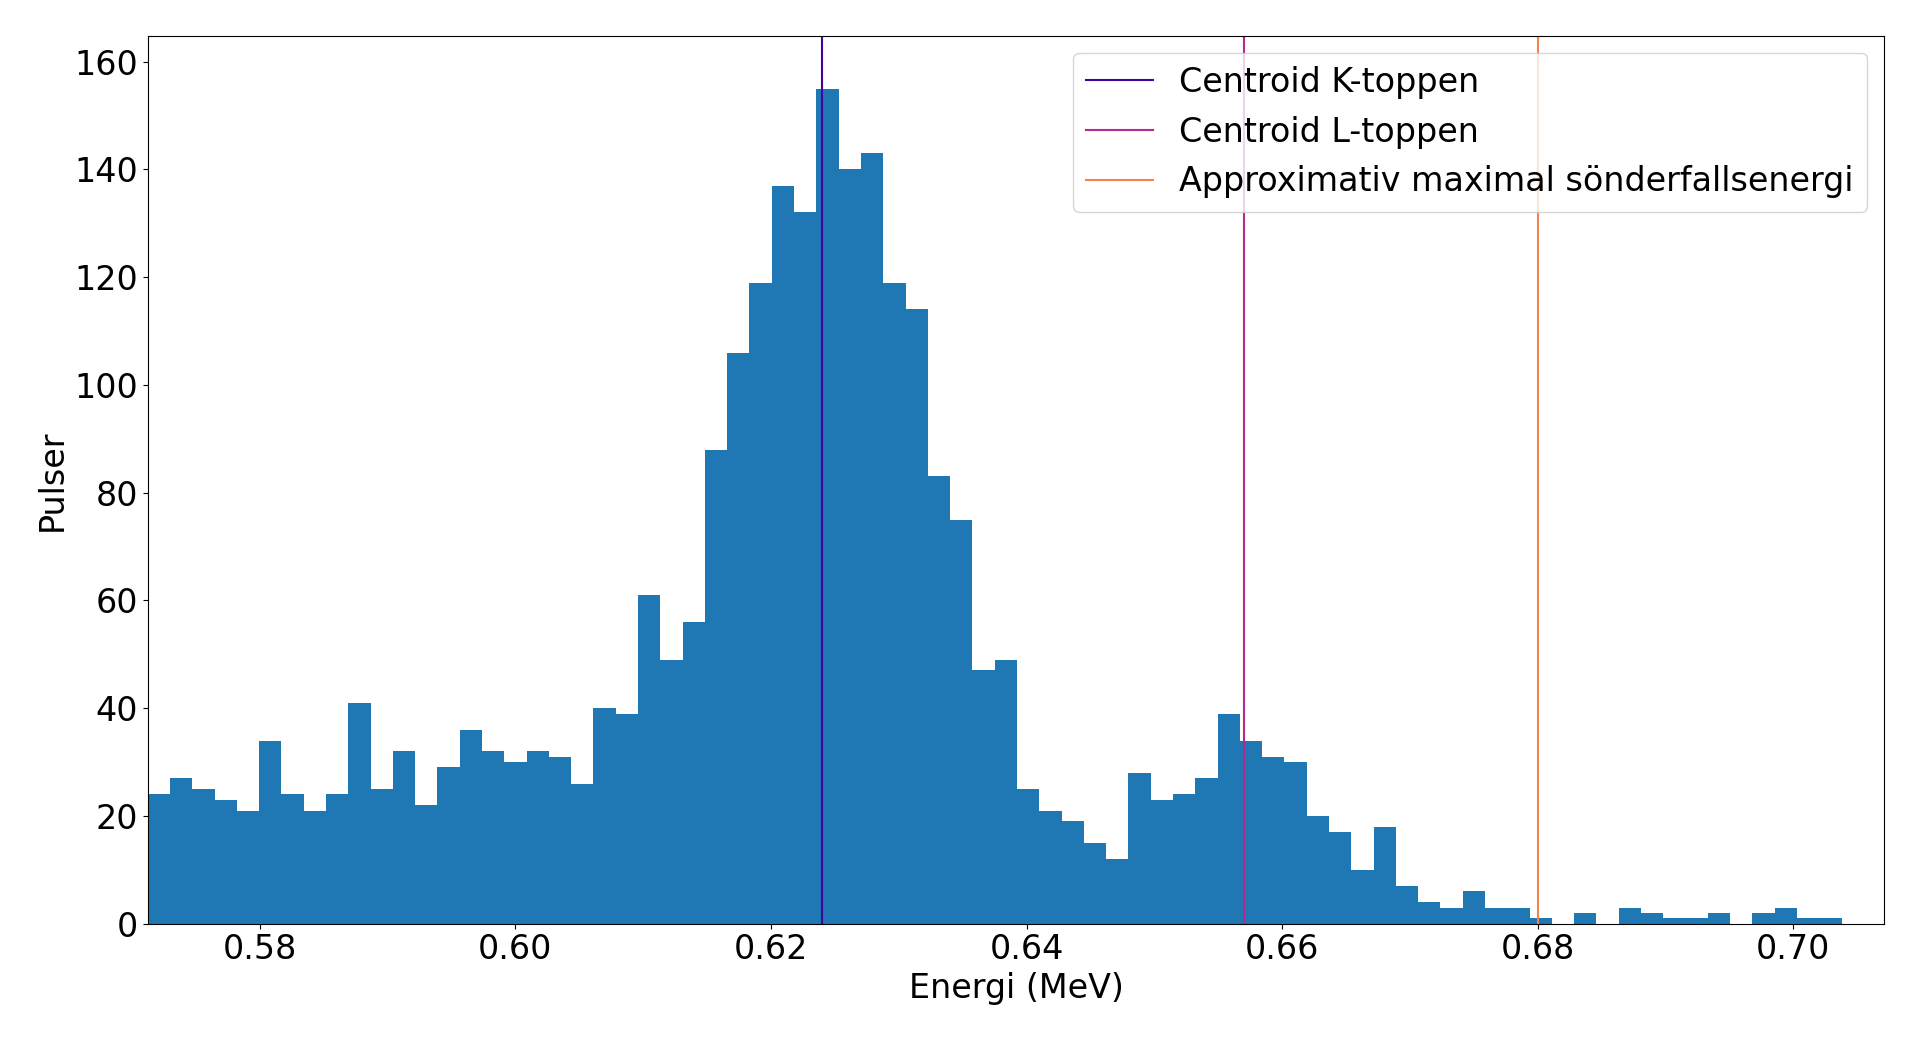
\includegraphics[width=\textwidth, keepaspectratio]{../images/cesium_max.png}
    \caption{
        Förstoring av högerkant av betaspektrum från figur~\ref{fig:cesium}.
        Uppmätt maximalt värde är markerat.
    }
    \label{fig:cesiummax}
\end{figure}
